\documentclass{tufte-book}

\hypersetup{colorlinks}% uncomment this line if you prefer colored hyperlinks (e.g., for onscreen viewing)

%%
% Book metadata
\title{Analytics}
\author[]{Sounds LAB}

%%
% If they're installed, use Bergamo and Chantilly from www.fontsite.com.
% They're clones of Bembo and Gill Sans, respectively.
%\IfFileExists{bergamo.sty}{\usepackage[osf]{bergamo}}{}% Bembo
%\IfFileExists{chantill.sty}{\usepackage{chantill}}{}% Gill Sans

%\usepackage{microtype}

%%
% Just some sample text
\usepackage{lipsum}

%%
% For nicely typeset tabular material
\usepackage{booktabs}

% for math
\usepackage{amsmath}

%%
% For graphics / images
\usepackage{graphicx}
\setkeys{Gin}{width=\linewidth,totalheight=\textheight,keepaspectratio}
\graphicspath{{graphics/}}

% The fancyvrb package lets us customize the formatting of verbatim
% environments.  We use a slightly smaller font.
\usepackage{fancyvrb}
\fvset{fontsize=\normalsize}

%%
% Prints argument within hanging parentheses (i.e., parentheses that take
% up no horizontal space).  Useful in tabular environments.
\newcommand{\hangp}[1]{\makebox[0pt][r]{(}#1\makebox[0pt][l]{)}}

%%
% Prints an asterisk that takes up no horizontal space.
% Useful in tabular environments.
\newcommand{\hangstar}{\makebox[0pt][l]{*}}

%%
% Prints a trailing space in a smart way.
\usepackage{xspace}

%%
% Some shortcuts for Tufte's book titles.  The lowercase commands will
% produce the initials of the book title in italics.  The all-caps commands
% will print out the full title of the book in italics.
\newcommand{\vdqi}{\textit{VDQI}\xspace}
\newcommand{\ei}{\textit{EI}\xspace}
\newcommand{\ve}{\textit{VE}\xspace}
\newcommand{\be}{\textit{BE}\xspace}
\newcommand{\VDQI}{\textit{The Visual Display of Quantitative Information}\xspace}
\newcommand{\EI}{\textit{Envisioning Information}\xspace}
\newcommand{\VE}{\textit{Visual Explanations}\xspace}
\newcommand{\BE}{\textit{Beautiful Evidence}\xspace}

\newcommand{\TL}{Tufte-\LaTeX\xspace}

% Prints the month name (e.g., January) and the year (e.g., 2008)
\newcommand{\monthyear}{%
  \ifcase\month\or January\or February\or March\or April\or May\or June\or
  July\or August\or September\or October\or November\or
  December\fi\space\number\year
}


% Prints an epigraph and speaker in sans serif, all-caps type.
\newcommand{\openepigraph}[2]{%
  %\sffamily\fontsize{14}{16}\selectfont
  \begin{fullwidth}
  \sffamily\large
  \begin{doublespace}
  \noindent\allcaps{#1}\\% epigraph
  \noindent\allcaps{#2}% author
  \end{doublespace}
  \end{fullwidth}
}

% Inserts a blank page
\newcommand{\blankpage}{\newpage\hbox{}\thispagestyle{empty}\newpage}

\usepackage{units}

% Typesets the font size, leading, and measure in the form of 10/12x26 pc.
\newcommand{\measure}[3]{#1/#2$\times$\unit[#3]{pc}}

% Macros for typesetting the documentation
\newcommand{\hlred}[1]{\textcolor{Maroon}{#1}}% prints in red
\newcommand{\hangleft}[1]{\makebox[0pt][r]{#1}}
\newcommand{\hairsp}{\hspace{1pt}}% hair space
\newcommand{\hquad}{\hskip0.5em\relax}% half quad space
\newcommand{\TODO}{\textcolor{red}{\bf TODO!}\xspace}
\newcommand{\na}{\quad--}% used in tables for N/A cells
\providecommand{\XeLaTeX}{X\lower.5ex\hbox{\kern-0.15em\reflectbox{E}}\kern-0.1em\LaTeX}
\newcommand{\tXeLaTeX}{\XeLaTeX\index{XeLaTeX@\protect\XeLaTeX}}
% \index{\texttt{\textbackslash xyz}@\hangleft{\texttt{\textbackslash}}\texttt{xyz}}
\newcommand{\tuftebs}{\symbol{'134}}% a backslash in tt type in OT1/T1
\newcommand{\doccmdnoindex}[2][]{\texttt{\tuftebs#2}}% command name -- adds backslash automatically (and doesn't add cmd to the index)
\newcommand{\doccmddef}[2][]{%
  \hlred{\texttt{\tuftebs#2}}\label{cmd:#2}%
  \ifthenelse{\isempty{#1}}%
    {% add the command to the index
      \index{#2 command@\protect\hangleft{\texttt{\tuftebs}}\texttt{#2}}% command name
    }%
    {% add the command and package to the index
      \index{#2 command@\protect\hangleft{\texttt{\tuftebs}}\texttt{#2} (\texttt{#1} package)}% command name
      \index{#1 package@\texttt{#1} package}\index{packages!#1@\texttt{#1}}% package name
    }%
}% command name -- adds backslash automatically
\newcommand{\doccmd}[2][]{%
  \texttt{\tuftebs#2}%
  \ifthenelse{\isempty{#1}}%
    {% add the command to the index
      \index{#2 command@\protect\hangleft{\texttt{\tuftebs}}\texttt{#2}}% command name
    }%
    {% add the command and package to the index
      \index{#2 command@\protect\hangleft{\texttt{\tuftebs}}\texttt{#2} (\texttt{#1} package)}% command name
      \index{#1 package@\texttt{#1} package}\index{packages!#1@\texttt{#1}}% package name
    }%
}% command name -- adds backslash automatically
\newcommand{\docopt}[1]{\ensuremath{\langle}\textrm{\textit{#1}}\ensuremath{\rangle}}% optional command argument
\newcommand{\docarg}[1]{\textrm{\textit{#1}}}% (required) command argument
\newenvironment{docspec}{\begin{quotation}\ttfamily\parskip0pt\parindent0pt\ignorespaces}{\end{quotation}}% command specification environment
\newcommand{\docenv}[1]{\texttt{#1}\index{#1 environment@\texttt{#1} environment}\index{environments!#1@\texttt{#1}}}% environment name
\newcommand{\docenvdef}[1]{\hlred{\texttt{#1}}\label{env:#1}\index{#1 environment@\texttt{#1} environment}\index{environments!#1@\texttt{#1}}}% environment name
\newcommand{\docpkg}[1]{\texttt{#1}\index{#1 package@\texttt{#1} package}\index{packages!#1@\texttt{#1}}}% package name
\newcommand{\doccls}[1]{\texttt{#1}}% document class name
\newcommand{\docclsopt}[1]{\texttt{#1}\index{#1 class option@\texttt{#1} class option}\index{class options!#1@\texttt{#1}}}% document class option name
\newcommand{\docclsoptdef}[1]{\hlred{\texttt{#1}}\label{clsopt:#1}\index{#1 class option@\texttt{#1} class option}\index{class options!#1@\texttt{#1}}}% document class option name defined
\newcommand{\docmsg}[2]{\bigskip\begin{fullwidth}\noindent\ttfamily#1\end{fullwidth}\medskip\par\noindent#2}
\newcommand{\docfilehook}[2]{\texttt{#1}\index{file hooks!#2}\index{#1@\texttt{#1}}}
\newcommand{\doccounter}[1]{\texttt{#1}\index{#1 counter@\texttt{#1} counter}}

% Generates the index
\usepackage{makeidx}
\makeindex

\begin{document}

% r.3 full title page
\maketitle

% r.5 contents
\tableofcontents

% r.9 introduction
\cleardoublepage
\chapter*{Introduction}

This sumarizes all the knowledge that we have accquired regarding A/B testing.

\chapter{Why being Bayesian?}
\label{chap:why_bayes}

Bayesian statistics are not self-evident in the field of A/B testing. Quite the contrary: for a very long
time, virtually all companies relied to frequentist statistics and p-value in order to draw conclusions from
their tests (AirBnB, Stakoverflow...). There's been a trend recently to go towards Bayesian methods to
interpret results (ABTasty, VWO...). Why?

The question is worth answering, as frequentist statistics are considered by most to be "easier" to use, while
Bayesian methods requires one to learn a new framework that is rarely taught at school. Here are a few
reaseons, most gathered from~\cite{Murphy2012}:


\begin{itemize}
  \item[\textbf{Confidence intervals are weird.}] Unlike Bayesian who define credible intervals based on the
    posterior distribution (thus on data only), the confidence interval is derived from the sampling
    distribution of the estimator. We condition on what is unknown, the parameter $\theta$, and average over
    future hypothetical data $\tilde{\mathcal{D}}$. This is counter-intuitive and can lead to very
    pathological situations. They can't be trusted.
  \item[\textbf{p-values, anyone?}]
  \item[\textbf{Likelihood principle}]
  \item[\textbf{It doesn't answer the interesting questions}]
\end{itemize}

\chapter{The Bayesian way}
\label{chap:Bayes}

\section{Correction for multiple variants: hierarchical models}

\section{Stopping rule}
\label{sec:Stopping rule}

\subsection{Highest Posterior Density Interval}

\subsection{Smallest interesting difference}

\subsection{Improvement}

\section{Bayesian Workflow}

The Bayesian workflow to model a set of data should consist of the following steps~\cite{Gabry2018}.

\begin{enumerate}
    \item Exploratory data analysis. Go deeper than simply plotting the data, look for hidden patterns that
      may biais a naive model.
    \item Choose a set of models.
    \item Check the models using fake data. In particular, judge of the adequacy of the priors using prior
      predictive checks (predicting all possible data points).
    \item Check the computation. Go beyond trace plots.
    \item Posterior predictive checks
    \item Comparison between the different models
\end{enumerate}

  \subsection{Check the model}

Prior predictive check.~\cite{Betancourt2018}
  
  \subsection{Computation diagnostics}

\begin{itemize}
    \item Trace plot
    \item $\hat{R}$ statistic
    \item Other things for HMC~\cite{Betancourt2017}
\end{itemize}


  \subsection{Posterior predictive checks}


\section{When to stop the experiment?}

Experiment can, in theory, run forever. Often, we stop them for pratical reasons (we need the result now), or
because we have seen something that seemed significant. Both can be valuable reasons, as we will see, but the
ideas somewhat need to be normalized an integrated into a decision framework.

The idea of stopping experiments early, when there is a 'statistically significant' result is not new, and is
often justified on the basis of it being a good tradeoff between statistical accuracy and speed in decision.
Yet, this leads to several pathological cases, and should be studied more deeply.

Now, assume that we do not want to fall into the trap of 'early peaking' and choose a stopping rule that only
depends on the data that have been gathered so far. How do we choose when to stop? Does it have to be
arbitrary? As we will see, although you always have to draw a line in the sand, you can build a framework so
that the choice you have to make does not seem very arbitrary, and matches the heuristics we usually use ("Hey,
we need to put this in production by next week").


Here is how a discussion between data and product people usually goes:\\

"Hey, did you have time to look at the results on the feature we rolled out last week? We'd really like to
push it in prod, or take it down for the next feature"

"I did. The results are promising, but not statistically significant yet. We need to wait a little longer."

"Ok, promising is good enough to me. We really don't have time to wait for this. Close it."

Two things went wrong in this discussion:

\begin{itemize}
  \item \textit{Never} tell anyone (not even me) about the current trend on the metric, unless the decision
    tree has decided to stop. Before the experiment is finished, the results have no meaning! (at least report
    the loss you were ready to accept by choosing the variant you did).
  \item Finishing a test before reaching significance does not make sense, as we will see.
\end{itemize}

Also, notice all the assumptions that are not spelled out:

\begin{itemize}
  \item There \textit{is} a constraint on the time an experiment can run, and we are not always ready to trade
    time for more accuracy. But how much are we ready to trade?
  \item There is a threshold of significance after which we feel we can stop the experiment. What is that
      threshold?
\end{itemize}

Clearly, there is a need to formalize and standardize the decision process. We'll see that this formalization
is not so much of a constraint---several parameters can be adjusted on an experiment basis---but it helps with
having a consistant decision protocol. Something that can be discussed in very specific terms.


We need to do a \textit{preposterior} analysis of the experiment design to minimize the overall cost. The
overall cost is the sum of the decision loss and the cost to run the experiment.

A sequential decision procedure is noted:

\begin{equation}
  \mathbf{d} = \left(\mathbf{\tau}, \mathbf{\delta}\right)
\end{equation}

where $\mathbf{\tau}_i$ is the probability to stop the experiment at stage $i$ and $\mathbf{\delta}_i$ is the
decision that has to be taken if the stop the experiment at stage $i$. It's often easier to speak in term of
\textit{stopping time} $N$:

\begin{equation}
  N = min\left\{n\geq0 | \mathbf{\tau}_n = 1\right\}
\end{equation}

The idea is that one should compare at every step the posterior Bayes risk of making a decision with the
"expected" Bayes risk that will be obtained if more observations are taken.



    \subsection{How bayesians make decisions}%
    \label{sub:how_bayesians_make_decisions}

- Loss
- Bayesian risk

    \subsection{The link with reinforcement learning}%
    \label{sub:the_link_with_reinforcement_learning}



\chapter{Models}
\label{chap:models}

  \section{Defining what a session is}%
  \label{sec:defining_what_a_session_is}
  
  
  \section{Subscription retention and lifetime value}%
  \label{sec:churn_of_subscription_and_lifetime_value}


    \subsection{Introduction: why it matters}%
    \label{sub:introduction_why_it_matters}
  
  
The churn of subscribers is defined in the following way. Let us note $N_0$ the number of users who subscribed
to a paid plan. We can measure the number of people $N_t$ who renewed their subscription at least until time
$t$. Taking all users of a same cohort, this gives us a list of integers:

\begin{equation}
  \left[N_0, \dots, N_T \right]
\end{equation}

where $T$ is the last observable time. Usually, we define a cohort as all the users who subscribed the same
month. Indeed, if we mix these cohorts we end with \textit{censored data}: some users who registered at time $0$
won't be present at time $T$ not because they churned, but because their subscription is not old enough. Once
should be aware of censored data, since they can introduce an important biais in the analysis.

Our goal in this section is to derive a model that describes the above list as well as possible. Why do we
care about modeling the churn? Mainly two reasons:

\begin{itemize}
  \item[\textbf{Financial forecasting}] A churn model would allow us to \textit{make predictions} about churn
    values in the future. That way, we are able to predict our future revenue. The Bayesian approach is
    crucial here as the model would allow to compute the \textit{uncertainty} on the future revenue. Point 
    predictions could be deadly here.
  \item[\textbf{Lifetime value}] Because we would be able to predict the number of users still paying after an
    arbitrary amount of time, we would be able to compute the lifetime value of subscribers in each plan. That
    way, we could adapt our marketing strategy towards the plans with the highest lifetime value. Also, this
    would let us know what is largest amount of money we can pay to acquire a paying user.
\end{itemize}

    \subsection{The model}%
    \label{sub:the_model}
 
We will use a generative model of the churn process. We assume that each subscriber $i$ has a probability
$\theta_i$ to cancel their subscription at any time. This probability is constant over time. This may seem odd
to marketers who tend to think that retention increases over time. We will see this observed increased can
simply be interpreted as a sorting effect.
We further assume that all the $\theta_i$ are drawn from the same Beta distribution with parameters $\alpha$
and $\beta$

\begin{equation}
  \theta_i \sim Beta(\alpha, \beta) \quad \forall i
\end{equation}

The parameters $\alpha$ and $\beta$ are descriptors of the application as a whole. We choose a Beta
distribution because it is a versatile distribution over $\left[0,1\right]$ that can take a variety of
different shapes as the values of $\alpha$ and $\beta$ vary.

We need to set a prior on $\alpha$ and $\beta$. We choose the weakly informative prior define by Gelman et al.
in~\cite{Gelman2014}:

\begin{equation}
  \alpha, \beta \sim \frac{1}{\left(\alpha+\beta\right)^{5/2}}
\end{equation}

The model is represented on Figure~\ref{fig:sbg}.

\begin{marginfigure}
  \centering
  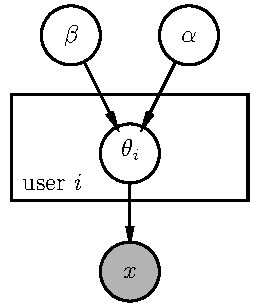
\includegraphics[width=\linewidth]{./figures/shifted_beta_geometric.pdf}
  \caption{Graphical representation of the subscription churn model. The vector $\mathbf{x}$ stands for the
  count data $[N, \dots, N_t]$.\label{fig:sbg}}
\end{marginfigure}

The number $n_t$ of users at an instant $t$ is given by

\begin{equation}
  n_t = \sum_{i=1}^N s_{it}
\end{equation}

where $s_{it}$ is the random variable equal to one when user $i$ is present at time $t$, and $0$ otherwise. It
is distributed according to:

\begin{align*}
  P(s_{it}=1) &\sim \left(1-\theta_i\right)^t\\
  P(s_{it}=0) &\sim \sum_{\tau=1}^t \theta_i \left(1-\theta_i\right)^{\tau-1}
\end{align*}

    \subsection{Inference}%
    \label{sub:inference}

Computing for all times $t$ in one go is complicated so we instead progress recursively. $s_{i1}$ is given by an
inverse Bernoulli distribution of parameter $\theta_i$. Since that, in absence of any further information, the
users are exchangeable, we have according to deFinetti's representation theorem:

\begin{equation}
  P(n_1 = N_1 | \vec{\theta}, \alpha, \beta) = \int_0^1 \theta_i^{N-N_1} \left(1-\theta_i\right)^{N_1}
  P(\theta_i|\alpha, \beta)\: \mathrm{d}\theta_i
\end{equation}

So, filling in the expression for $\theta_i$ conditional probability:

\begin{align}
  P(n_1=N_1) &= \int_0^1 \frac{\theta_i^{N-N_1+\alpha-1}\left(1-\theta_i\right)^{N_1+\beta-1}}{B(\alpha,
  \beta)}\:\mathrm{d}\theta_i \nonumber\\
  &= \frac{B(N-N_1+\alpha, N_1+\beta)}{B(\alpha, \beta)}
\label{sbg:recursion-formula}
\end{align}

The recursion is now obvious: it suffices to replace $N$ with $N_1$ and $N_1$ with $N_2$ to otbain
$P(n_2=N_2|n_1=N_1, n_0=N)$. The probability to observe $
\mathcal{D} = \left(n_0, n_1, \dots, n_t\right)$ if therefore:

\begin{align*}
  P(\mathcal{D} | \alpha, \beta) &= P(n_1|n_0, \alpha, \beta) P(n_1|n_2, n_1, \alpha, \beta) \dots\\
      &= \prod_{\tau=1}^t p(n_\tau|n_{\tau-1}, \alpha, \beta)
\end{align*}

\begin{marginfigure}
  \centering
  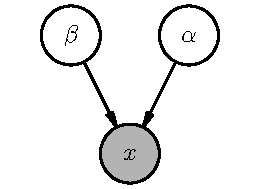
\includegraphics[width=\linewidth]{./figures/shifted_beta_geometric_marginalized.pdf}
  \caption{Marginalizing over $\theta$ gives the above graphical model. \label{fig:sbg}}
\end{marginfigure}

Therefore, following Bayes theorem:

\begin{equation}
  P(\alpha, \beta | \mathcal{D}) \propto \prod_{\tau=1}^t p(n_\tau|n_{\tau-1}, \alpha, \beta) P(\alpha, \beta)
\end{equation}


  \subsection{Prediction}%
  \label{sub:prediction}

Predict the number of individuals who will stay at ulterior periods for which we have no data. We only need to
use the recursion formula~\ref{sbg:recursion-formula} after having infered the distributions of $\alpha$ and
$\beta$. In practice, this means computing values recursively using the trace of $\alpha$ and $\beta$, which
gives a set of values for each point in time.

  
  \subsection{Lifetime Value}%
  \label{sub:lifetime_value}
  
Knowing the churn rate $\theta_i$ of a user $i$, the discount rate $d$ (which represents the `value of
time') and the price $m$ of the subscription, one can compute their lifetime value as:

\begin{equation}
  LTV_i = m \sum_{t=0}^\infty \frac{s_{it}}{\left(1+d\right)^t}
\end{equation}

Where $s_{it}$ is the random variable that is equal to $1$ if $i$ is present, $0$ otherwise. What we are interested in is the expected lifetime value of a user averaged over the possible values of
$\theta_1$

\begin{equation}
  E\left[LTV_i\right] = m \sum_{t=0}^\infty \frac{P(s_{it}=1|\theta_i)}{(1+d)^t}
\end{equation}

the total expected LTV is thus given by the integral over $\theta$ of the previous expression:

\begin{align*}
  E\left[LTV|\alpha, \beta\right] &= m \sum_{t=0}^\infty \left(\frac{1}{1+d}\right)^t \int_0^1 P(s_{it}=1 | \theta_i)
  P(\theta_i|\mathcal{D}, \alpha, \beta)
  \: \mathrm{d} \theta_i\\
  & = m \sum_{t=0}^\infty \left(\frac{1}{1+d}\right)^t \int_0^1 \left(1-\theta_i\right)^t P(\theta_i)
  \mathrm{d}\theta_i\\
  & = m \sum_{t=0}^\infty \left(\frac{1}{1+d}\right)^t \int_0^1 \frac{\left(1-\theta_i\right)^{\beta+t-1}
  \theta_i^{\alpha-1} }{B(\alpha, \beta)}\mathrm{d}\theta_i\\
  & = m \sum_{t=0}^\infty \left(\frac{1}{1+d}\right)^t \frac{Beta(\alpha, \beta+t) }{B(\alpha, \beta)}
\end{align*}

Using properties of the Beta and Gamma functions we have:

\begin{align*}
  \frac{Beta(\alpha, \beta+t)}{Beta(\alpha, \beta)} &=
  \frac{\Gamma(\alpha)\Gamma(\beta+t)\Gamma(\alpha+\beta)}{\Gamma(\alpha)\Gamma(\beta)\Gamma(\alpha+\beta+t)}\\
  &= \frac{\Gamma(\alpha+\beta)}{\Gamma(\beta)}
  \frac{(\beta+t-1)\dots\beta\:\Gamma(\beta)}{(\beta+\alpha+t-1)\dots(\alpha+\beta)\:\Gamma(\alpha+\beta)}\\
  &= \frac{(\beta+t-1)\dots\beta}{(\beta+\alpha+t-1)\dots(\alpha+\beta)}
\end{align*}

Using the Pochammer symbol notations $(\beta)_t = \beta \dots (\beta+t-1)$ and $(\alpha+\beta)_t =
(\alpha+\beta) \dots (
\alpha+\beta+t-1)$ we can write:

\begin{align*}
  E\left[LTV|\alpha, \beta\right] = m \sum_{t=0}^{\infty} \frac{(\beta)_t}{\left(\alpha+\beta\right)_t}
  \left(\frac{1}{1+d}\right)^t
\end{align*}

We use the trick $(1)_t = t!$ to write the expression in terms of the hypergeometric function:

$$
E\left[LTV | \alpha, \beta\right] = m \quad _2F_1(1; \beta; \alpha+\beta; 1/(1+d))
$$

\subsection{Using past data to infer recent LTV}

The issue when computing quantities such as lifetime value
  
\section{Retention and stickiness}
\label{sec:retention_and_stickiness}

\subsection{The Pareto/NBD model}
\label{sub:the_pareto_nbd_model}
In a non-contractual setting, the state of an user (churned or active)
cannot be observed. All the observations are related to \emph{past
  activities} of the user. From the observations of the time of past
activities, we need to estimate a probability of being active so that
we can project future retention.

The Pareto/NBD model is based on the following assumptions:
\begin{itemize}
\item The number of activities $x$ made in active period of length
  $t$ follows a Poisson distribution of mean $\lambda t$;
\item Heterogeneity in parameter $\lambda$ across users follows a
  gamma distibution of shape $r$ and scale $\alpha$;
\item The lifetime $\tau$ follows an exponential distribution of
  dropout rate $\mu$;
\item The heterogeneity in parameter $\mu$ across users follows a
  gamma distribution of shape $s$ and scale $\beta$;
\item $\lambda$ and $\mu$ are independent.
\end{itemize}

So formally:
\begin{align*}
x & \sim \frac{\lambda^x t^x e^{-\lambda t}}{x !} \\
\tau & \sim \mu e^{-\mu \tau} \\
\lambda & \sim Gamma(r,\alpha) \\
\mu & \sim Gamma(s, \beta)
\end{align*}

We are going to use variational inference methods to estimate the
parameters $r,\alpha, s, \beta$.

\subsection{Likelihood of the Pareto/NBD}
\label{sub:likelihood_of_the_pareto_nbd}

The number $x$ of events occuring in time $T$ follows a Poisson
distribution of rate $\lambda T$ iff the intervent times are
\emph{i.i.d.}  variables following an exponential distribution of rate
$\lambda$. That is to say the events times $0=t_0 < t_1 < \ldots < t_x
<T$ are such that:
$$t_i - t_{i-1} \sim \lambda e^{-\lambda (t_i - t_{i-1})} \qquad
i=1,\ldots,x $$

It is known that the distribution of $t_x$, the sum of $x$
exponentially distributed intervent times, is:
\begin{align*}
  t_x \sim \frac{\lambda^x t_x^{x-1} e^{-\lambda t_x}}{(x-1)!}
\end{align*}


Observing $x,t_x, T$ leaves us with two possibilities:
\begin{itemize}
\item the user is still active at time $T$ with no events between
  $t_x$ and $T$ (with probability $e^{-\lambda (T-t_x)} e^{-\mu T}$);
\item he has stopped being active at time
  $\tau \in \left] t_x, T \right]$ with no event between $t_x$ and
  $\tau$.
\end{itemize}
That is to say (for $x\ne 0$):
\begin{align*}
  P(x,t_x,T \ |\ \lambda, \mu) & = \frac{\lambda^x t_x^{x-1}
    e^{-(\lambda + \mu) T}}{(x-1)!} + \int_{t_x}^T \frac{\lambda^x
    t_x^{x-1} e^{-\lambda\tau}}{(x-1)!} \mu e^{-\mu \tau}
  \mathrm{d}\tau \\ & = \frac{\lambda^x t_x^{x-1} e^{-(\lambda + \mu)
      T}}{(x-1)!}  + \frac{\mu\lambda^x t_x^{x-1} \left(
    e^{-(\lambda+\mu)t_x} -e^{-(\lambda+\mu)T}\right)}{(\lambda + \mu)
    \times(x-1)!}\\ & = \frac{\lambda^x t_x^{x-1} \left( \lambda
    e^{-(\lambda+\mu)T}+ \mu e^{-(\lambda+\mu)t_x} \right)}{(\lambda +
    \mu) \times(x-1)!}
\end{align*}
And observing $(0,0,T)$ happens either when the user is still active at
time $T$ with no events within $T$ (with probability
$e^{-\lambda T} e^{-\mu T}$), or he has stopped being active at
time $\tau \in \left ] 0, T \right]$ with no event between $t_x$ and
$\tau$; that is to say:
\begin{align*}
  P(0,0,T \ |\ \lambda, \mu)
  & =  e^{-(\lambda + \mu) T}  + \int_{0}^T  e^{-\lambda\tau}    \mu e^{-\mu \tau}
    \mathrm{d}\tau \\
  & =
    \left(1 + \frac{\mu}{\lambda + \mu}\right)
    e^{-(\lambda + \mu) T}
\end{align*}

In~\cite{Schmittlein1987} an explicit likelihood of $x,t_x,T$
depending on $r,\alpha, s, \beta$ (where $\lambda$ and $\mu$ are
marginalised) is derived.\sidenote{It seems the likelihood derived
  in~\cite{Fader2005} contains an error.} However this expression is
complex and doesn't allow for explicit differentiation, preventing us
from using NUTS sampler. However the independence assumed between
$\lambda$ and $\mu$ makes variational inference suitable.


\subsection{Prediction}
\label{sub:prediction_pareto_nbd}

From the technical annex to~\cite{Abe2009}, we give a couple of
predictive probabilities which can be used for model-checking and
retention projection.

\paragraph{Survival probability}
\label{par:survivalprobability}

\begin{align*}
  P(\tau > T \ | \ \lambda, \mu, x, t_x, T)
  & = \frac{P(x, t_x, T \ | \ \lambda, \mu, \tau>T) P(\tau>T)}{
    P(x, t_x, T\ |\ \lambda, \mu)}\\
  & = \frac{1}{1+\frac{\mu}{\lambda+\mu}\left(
    e^{(\lambda+\mu)(T-t_x)}-1\right)}
\end{align*}


\paragraph{Expected activites in future period}
\label{par:expectedactivtiesinperiod0t}

Let $X(t_1, t_2)$ be the number of activities in the period $[t_1,t_2]$ for a
given user; then:
\begin{align*}
  E[X(0,t)\ |\ \lambda, \mu]
  & = \int_0^t \lambda\tau\mu e^{-\mu \tau} \mathrm{d}\tau
    + \lambda t e^{-\mu t} \\
  & = \frac{\lambda}{\mu} \left(e^{-\mu t} - 1\right)
\end{align*}
So, writing $\boldsymbol\theta = x, t_x, T, \lambda, \mu$, we get:
\begin{align*}
  E[X(T,T+t) \ | \ \boldsymbol\theta]
  & = E[X(0,t)\ | \ \lambda,\mu]
    P(\tau >T \ | \ \boldsymbol\theta)
\end{align*}



  
\section{Impact of new features on retention}

The impact of new features on retention is not something that is obvious to
measure. When one performs a naive A/B test, where one variant contains the
feature and the other one doesn't, the question that is being answered when
comparing the retention of the two cohorts is:

\begin{quotation}
	What is the average difference in terms of retention between users who
	can potentially see and use the feature and those who can't.
\end{quotation}

However, this is not the question we are interested in. Instead, what we would
like to know is:

\begin{quotation}
    1. Of all the people who have seen the feature, how many have used it?\\
    2. Does knowing that the feature exists influence the retention?\\
    3. Does using the feature influence the retention?
\end{quotation}

Ultimately, only question (2) requires an A/B test to be answered (unless,
arguably, when the feature is hidden and it is possible to use the application
without seeing it).

For individuals in the cohort that cannot access the feature, te

\chapter{The future}
\section{Multi-armed bandits}

\section{Can we learn faster?}

Can we reach statistical significance earlier?

https://erikbern.com/2017/12/12/learning-from-users-faster-using-machine-learning.html

\section{Just for fun: a short review of inference methods}

\subsection{Variational Inference}

\section{Monte Carlo Sampling}


Hamiltonian Monte Carlo~\cite{Betancourt2017}.

Riemannian Monte Carlo~\cite{Betancourt2013}


%%
% Start the main matter (normal chapters)
\mainmatter

%%
% The back matter contains appendices, bibliographies, indices, glossaries, etc.







\backmatter

\bibliography{references}
\bibliographystyle{plainnat}

\printindex

\end{document}

